%----------------------------------------------------------------------------------------
%    PACKAGES AND THEMES
%----------------------------------------------------------------------------------------

\documentclass[aspectratio=169,xcolor=dvipsnames]{beamer}
\usetheme{SimplePlus}

\usepackage{tikz}
\usepackage{hyperref}
\usepackage{graphicx} % Allows including images
\usepackage{booktabs} % Allows the use of \toprule, \midrule and \bottomrule in tables
\usepackage{amsmath}

%----------------------------------------------------------------------------------------
%    TITLE PAGE
%----------------------------------------------------------------------------------------

\title{Motivations for Predictive Analytics \& Machine Learning}
\subtitle{HI 743}

\author{Ryan Gallagher}

\institute
{
    Department of Health Informatics and Administration \\
    Zilber College of Public Health \\
    University of Wisconsin - Milwaukee% Your institution for the title page
}
\date{January 30, 2025} % Date, can be changed to a custom date

%----------------------------------------------------------------------------------------
%    PRESENTATION SLIDES
%----------------------------------------------------------------------------------------

\begin{document}

\begin{frame}
    % Print the title page as the first slide
    \titlepage
\end{frame}
%------------------------------------------------

%\begin{frame}{Overview}
    % Throughout your presentation, if you choose to use \section{} and \subsection{} commands, these will automatically be printed on this slide as an overview of your presentation
%    \tableofcontents
%\end{frame}
%------------------------------------------------

\section{}
\begin{frame}{Machine Learning for Predictive Analytics}
Modern organizations collect massive amounts of data. For data to be of value to an organization, they must be analyzed to \textbf{extract insights that can be used to make better decisions}. Extracting insights from data is the job of data analytics. 
\vspace{1cm}
\begin{center}
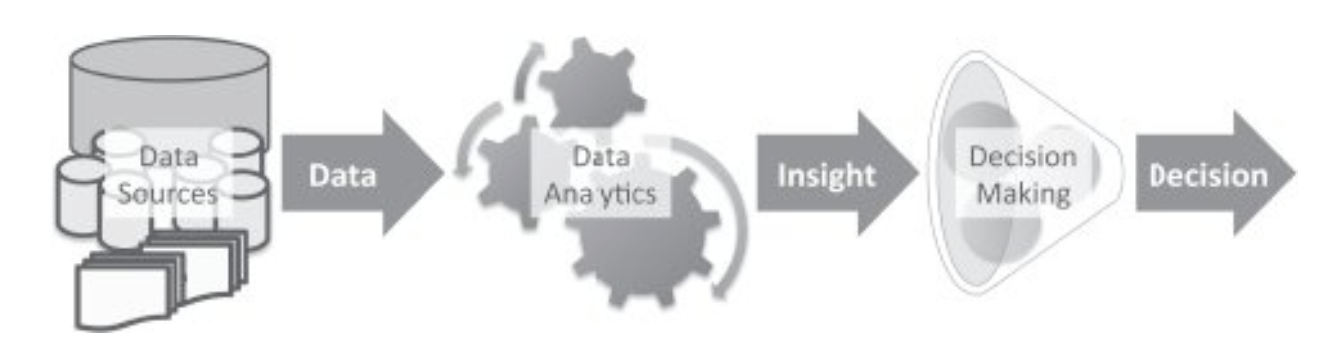
\includegraphics[scale=0.5]{images/fig1.1.png}
\end{center}

% Notes:
% Mention my experiences (WPS, EMR Research, Genomics) and relate that to this figure.
%  An analyst must be the interpreter of data for those who are positioned to make decisions.

\end{frame}

%------------------------------------------------

\begin{frame}{What is Predictive Analytics?}
\textbf{Predictive data analytics} is the art of building and using models that make predictions based on patterns extracted from historical data. Applications of predictive data analytics include:

\begin{itemize}
	\item \textbf{Dosage Prediction}: Doctors and scientists frequently decide how much of a medicine or other chemical to include in a treatment. Predictive analytics models can be used to assist this decision making by predicting optimal dosages based on data about past dosages and associated outcomes.
	
	\item \textbf{Diagnosis}: Doctors, engineers, and scientists regularly make diagnoses as part of their work. Typically, these diagnoses are based on their extensive training, expertise, and experience. Predictive analytics models can help professionals make better diagnoses by leveraging large collections of historical examples at a scale beyond anything one individual would see over his or her career. The diagnoses made by predictive analytics models usually become an input into the professional’s existing diagnosis process.

\end{itemize}
\end{frame}

%------------------------------------------------


\begin{frame}{What is Predictive Analytics?}
\begin{itemize}
	\item \textbf{Document Classification}: Predictive data analytics can be used to automatically classify documents into different categories. Examples include email spam filtering, news sentiment analysis, customer complaint redirection, and medical decision making. In fact, the definition of a document can be expanded to include images, sounds, and videos, all of which can be classified using predictive data analytics models.
\end{itemize}
\vspace{0.5cm}
In each case a model is used to make a prediction to help a person or organization make a decision. In predictive data analytics \textbf{we use a broad definition of the word prediction}. In everyday usage, the word prediction has a temporal (time) aspect—we predict what will happen in the future. However, \textbf{in data analytics a prediction is the assignment of a value to any unknown variable}. The examples listed above are trained to make predictions based on a set of historical examples. We use machine learning to train these models.

\end{frame}

%------------------------------------------------


\begin{frame}{What is Machine Learning?}
\begin{itemize}
\setlength{\itemsep}{.25cm}
\item Machine learning is defined as an \textbf{automated process that extracts patterns from data}. To
build the models used in predictive data analytics applications, we use supervised
machine learning.

\item Supervised machine learning involves building a statistical model for predicting, or estimating, an \textit{output} based on one or more \textit{inputs}.

\item With unsupervised machine learning, there are inputs but \textit{no supervising output}; nevertheless we can learn relationships and structure within the data.
\end{itemize}
\end{frame}

%------------------------------------------------

\begin{frame}{Application Example: Wage Data}

In our text, we're given the \texttt{Wage} dataset which examines a number of factors that relate to wages for a group of men from the Atlantic region of the United States. We wish to understand the association between an employee’s age and education, as well as the calendar year, on his wage.
\vspace{.5cm}
% notes on the interpretation and take-aways:
% Wage data, which contains income survey information for men from the central Atlantic region of the United States. Left: wage as a function of age. On average, wage increases with age until about 60 years of age, at which point it begins to decline. Center: wage as a function of year. There is a slow but steady increase of approximately $10,000 in the average wage between 2003 and 2009. Right: Boxplots displaying wage as a function of education, with 1 indicating the lowest level (no high school diploma) and 5 the highest level (an advanced graduate degree). On average, wage increases with the level of education.

\begin{center}
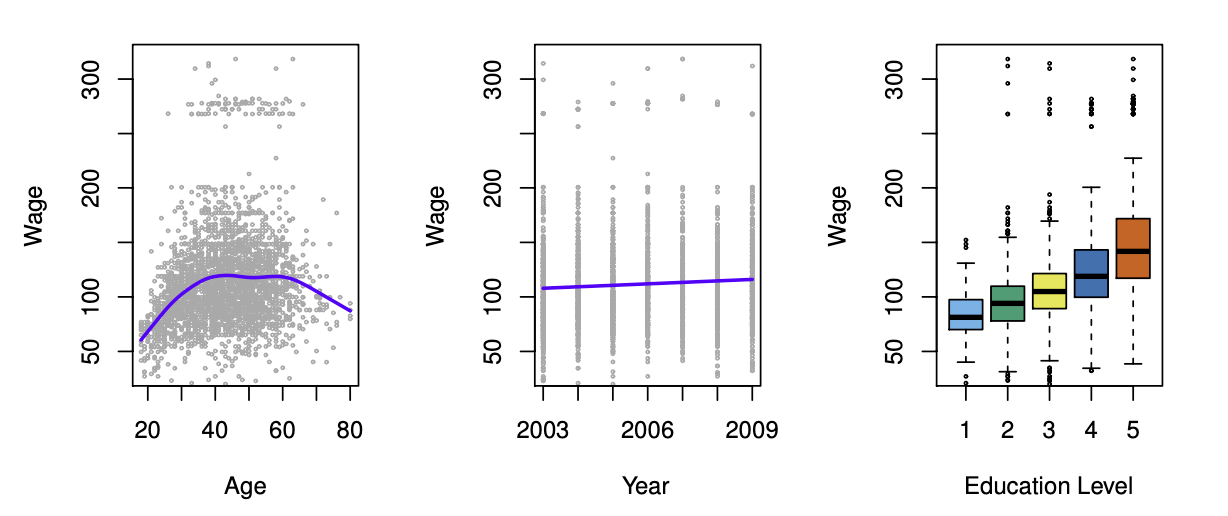
\includegraphics[scale=0.5]{images/wage_figs.png}
\end{center}

\end{frame}

%------------------------------------------------

\begin{frame}{Application Example: Gene Expression}
Also in our text, we're given the NCI60 data set, which consists of 6,830 gene expression measurements for each of 64 cancer cell lines. Instead of predicting a particular output variable, we are interested in determining whether there are groups, or clusters, among the cell lines based on their gene expression measurements.

\begin{center}
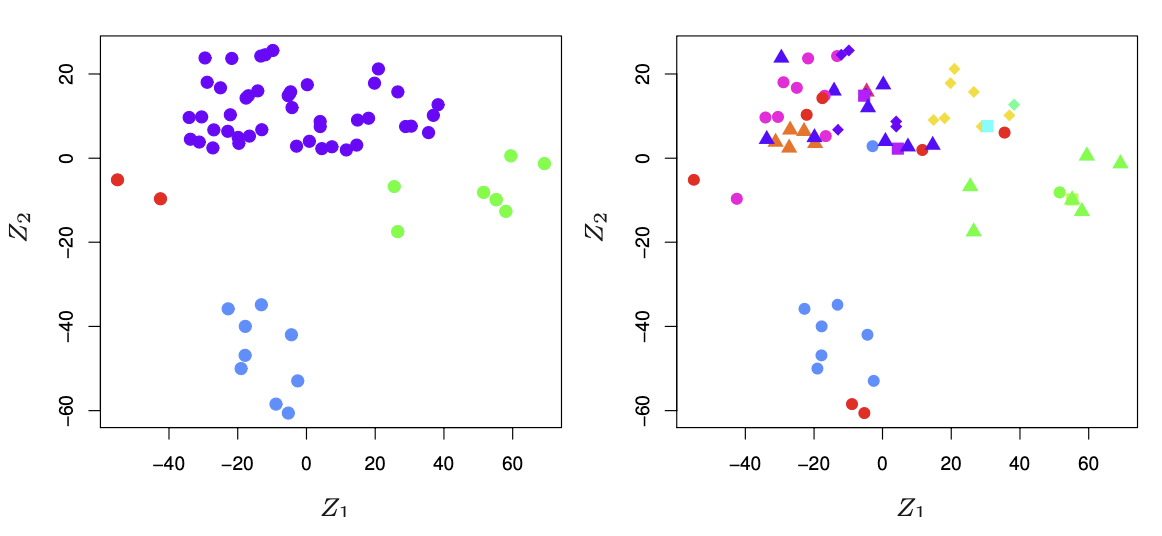
\includegraphics[scale=0.4]{images/gene_expr.png}
\end{center}

%Left: Representation of the NCI60 gene expression data set in a two-dimensional space, Z1 and Z2. Each point corresponds to one of the 64 cell lines. There appear to be four groups of cell lines, which we have represented using different colors. Right: Same as left panel except that we have represented each of the 14 different types of cancer using a different colored symbol. Cell lines corresponding to the same cancer type tend to be nearby in the two-dimensional space.

\end{frame}

%------------------------------------------------


\begin{frame}{How Does Machine Learning Work?}
\begin{itemize}
\setlength{\itemsep}{.25cm}

\item Machine learning algorithms work by searching through a set of possible prediction models for the model that best captures the relationship between the \textit{descriptive features} and \textit{target feature} in a dataset.

\item A prediction model that makes the correct predictions for these queries captures the underlying relationship between the descriptive and target features and is said to \textbf{generalize} well.

\item The goal of machine learning is to find the predictive model that generalizes best by using some criteria for choosing among the candidate models it considers during its search.


\end{itemize}
\end{frame}

%------------------------------------------------


\begin{frame}{How Does Machine Learning Work?}
\begin{itemize}
\setlength{\itemsep}{.5cm}

\item The criterion to select the best prediction model is why there are a lot of different machine learning algorithms. When we choose to use one machine learning algorithm, we are choosing to use one model selection criterion over another.

\item All the different model selection criteria consist of a set of assumptions about the characteristics of the model that we would like the algorithm to induce. The set of assumptions that defines the model selection criteria of a machine learning algorithm is
known as the \textbf{inductive bias} of the machine learning algorithm.

\end{itemize}
\end{frame}

%------------------------------------------------


\begin{frame}{How Does Machine Learning Work?}
\begin{itemize}
\setlength{\itemsep}{.5cm}

\item There are two types of \textbf{Inductive Bias}:
	\begin{itemize}
	\item \textbf{Restriction Bias}: constrains the set of models allowed for the algorithm to consider.
	\item \textbf{Preference Bias}: guides the algorithm to prefer certain models over others.
	\end{itemize}
\end{itemize}
\vspace{.5cm}
In summary, machine learning works by searching through a set of potential models to find the prediction model that best generalizes beyond the dataset. Machine learning algorithms use two sources of information to guide this search, the training dataset and the inductive bias assumed by the algorithm.

\end{frame}

%------------------------------------------------


\begin{frame}{How Does Machine Learning Work?}
\begin{itemize}
\setlength{\itemsep}{.25cm}

\item \textbf{Prediction:} In many situations, a set of inputs X are readily available, but the output Y cannot be easily obtained. $$\hat{Y} = \hat{f}(X)$$
where $\hat{f}$ represents our estimate for f, and $\hat{Y}$ represents the resulting prediction for Y.
\item The accuracy of $\hat{Y}$ as a prediction for Y depends on two quantities, which we will call the \textit{reducible error} and the \textit{irreducible error} (or \textit{noise}).
\end{itemize}
% Reducible error reduced by a better model
% Irreducible error caused by unknown variables or elements outside of out data.

\end{frame}

%------------------------------------------------

\begin{frame}{How Does Machine Learning Work?}
\begin{itemize}
\setlength{\itemsep}{.25cm}

\item Consider a given estimate $\hat{f}$ and a set of predictors X, which yields the prediction $\hat{Y} = \hat{f}(X)$. Assume for a moment that both $\hat{f}$ and X are fixed, so that the only variability comes from $\epsilon$.

\begin{align*}
E(Y - \hat{Y})^2 &= E[f(X) + \epsilon - \hat{f}(X)]^2 \\
&= \underbrace{[f(X) - \hat{f}(X)]^2}_{\text{Reducible}} + \underbrace{Var(\epsilon)}_{\text{Irredicuble}}
\end{align*}

\item Machine Learning focuses on techniques for estimating $f$ with the aim of \textbf{minimizing the reducible error}. It is important to remember that the irreducible error will always maintain an upper bound on the accuracy of our prediction for $Y$. This bound is almost always unknown in practice.

\end{itemize}
\end{frame}

%------------------------------------------------

\begin{frame}{How Does Machine Learning Work?}
\begin{itemize}
\setlength{\itemsep}{.25cm}
	\item \textbf{Inference}: We still wish to estimate $f$, but are not necessarily trying to make predictions for $Y$. In this setting, we might be interested in answering the following questions:
	\begin{itemize}
	\setlength{\itemsep}{.2cm}
		\item \textit{Which predictors are associated with the response?} \\
		Identifying the few \textbf{important} predictors among a large set can be extremely useful.
		\item \textit{What is the relationship between the response and each predictor?} \\
		Some predictors may have positive/negative relationships with $Y$. 
		%Depending on the complexity of $f$, the relationship between $Y$ and a given predictors may depend on the values of other predictors.
		\item \textit{Can the relationship between Y and each predictors be adequately summarized using a linear equation, or is it more complex?}
	\end{itemize}

\end{itemize}
\end{frame}

%------------------------------------------------
\begin{frame}{The Accuracy \& Interpretability Trade-Off}
\begin{itemize}
\setlength{\itemsep}{.25cm}

\item When inference is the goal we would prefer using simple and relatively inflexible machine learning methods. In some settings, however, we may only be interested in prediction, and the interpretability of the predictive model is simply not of interest.
%Least squares linear regression is relatively inflexible but is quite interpretable.

%The lasso  relies upon the linear model (2.4) but uses an alternative fitting procedure for estimating the coefficients. The new procedure is more restrictive in es- timating the coefficients, and sets a number of them to exactly zero. Hence in this sense the lasso is a less flexible approach than linear regression.

% Generalized additive models (GAMs) instead extend the linear model (2.4) to allow for certain non-linear relationships. GAMs are more flexible than linear regression.

% Finally, fully non-linear methods such as bagging, boosting, support vector machines with non-linear kernels, and neural networks (deep learning) are highly flexible approaches that are harder to interpret.
\end{itemize}
\begin{center}
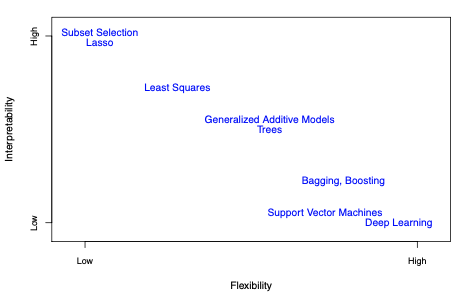
\includegraphics[scale=0.5]{images/trade_off.png}
\end{center}
\end{frame}

%------------------------------------------------

\begin{frame}{Assessing Model Accuracy}
\begin{itemize}
\setlength{\itemsep}{.25cm}
\item As previously mentioned, model selection consists of a set of assumptions where we seek to find the best fit for the data \& our question. Selecting the best approach can be one of the most challenging parts of performing statistical learning in practice.

\item A classic quantitative approach to measuring model-fit in the \textbf{regression} setting is \textit{mean squared error} (MSE):
$$MSE = \frac{1}{n}\sum^{n}_{i=1} (y_i - \hat{f}(x_i))^2$$
\end{itemize}
In regression settings, we can fit a model to the \textit{training data} and assess then test the model by obtaining the the \textit{test MSE}. This will be explored in our Error Based Machine Learning module.
\end{frame}

%------------------------------------------------

\begin{frame}{Assessing Model Accuracy}
\begin{itemize}
\setlength{\itemsep}{.25cm}

\item A quantitative approach to measuring model-fit in the \textbf{classification} setting is the \textit{error rate}:
$$ER = \frac{1}{n}\sum^{n}_{i=1} (y_i \neq \hat{y}_i))^2$$
\end{itemize}
In the classification settings, this is a simple proportion statistic that measures how observations where were incorrectly classified using the proposed model. This will be explored further in our Classification module. 
\end{frame}

%------------------------------------------------
\begin{frame}{What Can Go Wrong with Machine Learning?}
\begin{itemize}
\setlength{\itemsep}{.25cm}

\item There are two kinds of mistakes that an inappropriate inductive bias can lead to:
	\begin{itemize}
	\item \textbf{Underfitting}: occurs when the prediction model selected by the algorithm is too simplistic to represent the underlying relationship in the dataset between the descriptive features and the target feature.
	\item \textbf{Overfitting}: occurs when the prediction model selected by the algorithm is so complex that the model fits to the dataset too closely and becomes sensitive to noise in the data.
	\end{itemize}
\begin{center}
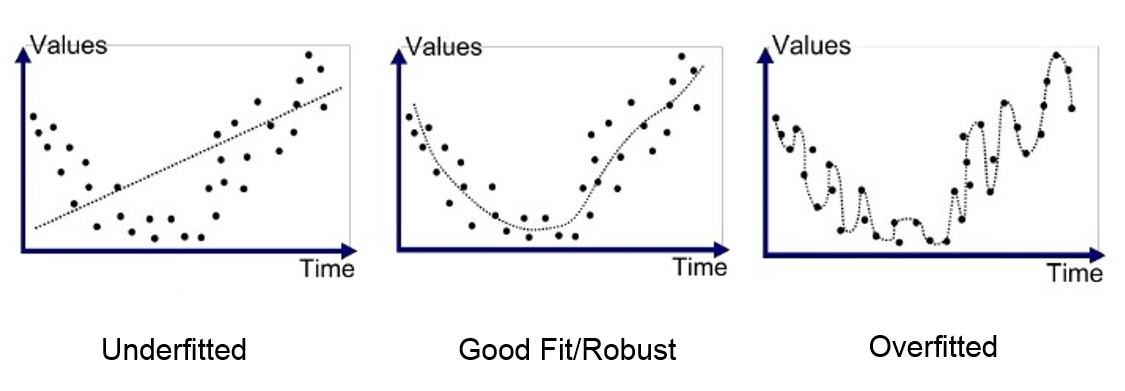
\includegraphics[scale=0.3]{images/fitting.png}
\end{center}
\end{itemize}
\end{frame}

%------------------------------------------------

\begin{frame}{Predictive Analytics Project Lifecycle: CRISP-DM}
\begin{itemize}
\setlength{\itemsep}{.25cm}

\item Our text describes a widely adopted predictive analytics project framework, \textbf{CRIPS-DM}: CRoss Industry Standard Process for Data Mining.

\item This framework is non-proprietary and industry/application neutral. It's a good way to look at a project from an objectively analytical point of view. \\ (\href{https://almirgouvea.github.io/The-Crisp-DM-Methodology/chapters/intro.html}{\color{blue} Methodology Handbook Link})
\begin{center}
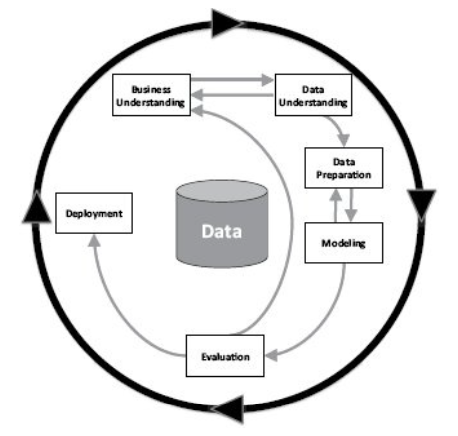
\includegraphics[scale=0.3]{images/crisp-dm.png}
\end{center}
\end{itemize}
\end{frame}

%------------------------------------------------
\begin{frame}{Predictive Analytics Project Lifecycle: CRISP-DM}
\begin{center}
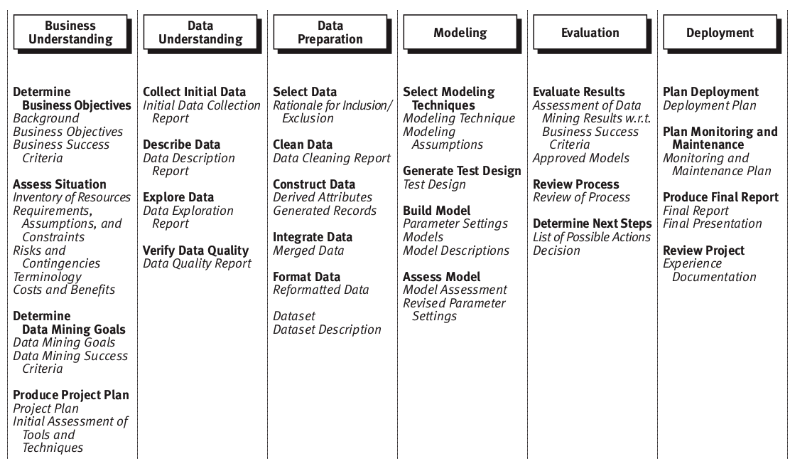
\includegraphics[scale=0.45]{images/crisp-dm-fig.png}
\end{center}
\end{frame}

%------------------------------------------------

\begin{frame}{Predictive Analytics Tools}
There are multiple applications which are capable of importing, preparing, modeling, and interpreting data.
\vspace{.2cm}
\begin{itemize}
\setlength{\itemsep}{.25cm}
\item \textbf{Application-based Tools}: IBM SPSS, Knime Analytics, SAS Enterprise, Weka, Excel
\item \textbf{Programming Languages}: \textit{R}, Python, SAS, SQL
\end{itemize}
\vspace{.2cm}
This course will be partial towards programming languages, particularly \textit{R}. \textit{R} is robust, well maintained, and highly adopted within the data analytics industry. 
\end{frame}

%------------------------------------------------
\begin{frame}{For Next Time: Download \& Install \textit{R}}
\begin{itemize}
\setlength{\itemsep}{.5cm}
\item \textbf{Install \textit{R}}: Follow the installation instructions at {\color{blue}https://cran.rstudio.com/}
\begin{itemize}
\setlength{\itemsep}{.25cm}
	\item \textbf{Windows Users:} Follow {\color{blue}\underline{Download R for Windows}} link $\rightarrow$ Download {\color{blue}\underline{base}} $\rightarrow$ Follow installation wizard.
	\item \textbf{macOS Users:} Follow {\color{blue}\underline{Download R for macOS}} $\rightarrow$ Select {\color{blue}\underline{.pkg}} for your processor type (Apple Silicon vs. Intel) $\rightarrow$ Follow installation wizard.
\end{itemize}
\item \textbf{Install RStudio}: Instruction at {\color{blue}https://posit.co/download/rstudio-desktop/}
\begin{itemize}
	\item This website should detect your operating system. Big blue button should say \texttt{Download Rstudio Desktop for \{Your OS\}}.
\end{itemize}
\end{itemize}
\vspace{0.5cm}
(\href{https://www.youtube.com/watch?v=fJS6iYeSDTM}{\color{blue} Windows Install Tutorial})
\hspace{6cm}
(\href{https://www.youtube.com/watch?v=sjcPE7Jbzbg}{\color{blue} macOS Install Tutorial})
\end{frame}



\end{document}